% !TEX root = template.tex
\section{Experimental Setup}

\subsection{Signals and Features}
\label{sec:sig&features}

%Com'è , il dataset, che tipo di features uso, spiegare come sono estratte, spiegare augmentation strategies, spiegare come genero gli split del dataset per ogni task.

Each model was trained on the Google Speech Commands dataset V2 \cite{speechdataset2018warden}, which consists on a total of $105829$ user utterances of a total of $35$ keywords. Each utterance is stored as a one second long\footnote{Some clips are a bit shorter than one second: in those cases, the clips are zero padded towards the end.} \verb|WAVE| file, sampled at a 16KHz rate. From each signal, $40$ MFCCs are computed, using a window size of $25$\textit{ms} ($400$ samples) and a hop size of $10$\textit{ms} ($160$ samples). With this approach, the input for the network consists in 3D tensors with one outer channel, where width represents the time domain and height represents the frequency domain. Following Google's suggestions from \cite{speechdataset2018warden}, the dataset is split in 80\% for training set, 10\% for validation set and 10\% for test set, in such a way that the same speakers are never present in two different splits. 
Following the approach from past literature, the models are trained for two different tasks, which are the following:
\begin{itemize}
	\item \textbf{12kws} task: the model must discriminate among 12 different keywords: \say{yes}, \say{no}, \say{up}, \say{down}, \say{left}, \say{right}, \say{on}, \say{off}, \say{stop}, \say{go}, unknown or silence. The unknown keywords are randomly chosen from the set of remaining keywords and the silence samples consist in one second long crops, randomly extracted from the noise files provided by the dataset\footnote{Those consist in 6 files containing noisy background sounds, both artificially generated and recorded from real environments.}. Since the total amount of words belonging to the \say{unknown} class was much more than number of representatives for each of the other keywords, we decided to randomly extract them to create a balanced dataset. In this way, we have 36921 samples for training, 4443 for validation and 4888 for testing.
	\item \textbf{35kws} task: the model must discriminate among all the 35 keywords present in the dataset. No unknown class or silence class is introduced, therefore, for this task, the entire dataset is used. The training set consists in 84843 samples, the validation set in 9981 samples and the test set in 11005 samples. 
\end{itemize}


For each task, the training set is augmented, following existing approaches from the literature. Specifically, the augmentation process follows this order:
\begin{enumerate}
	\item Each signal is randomly shifted left or right (zero padding the remaining portion), by $x$ samples, where $x$ is drawn from a uniform distirbution $U(0,100)$;
	\item Samples belonging to the \say{silence} class do not remain the same across epochs, but are randomly generated each time;
	\item With a probability of $0.8$, each signal is mixed with a randomly generated background noise, which is multiplied by a factor drawn from $U(0,0.2)$; 
	\item After the conversion in MFCC, the features are augmented using SpecAugment \cite{park2019specaugment}, a simple data augmentation method which consists in adding randomly sized frequency and time masks to the feature matrix: this is done in order to render the model more robust to partial loss of frequency information or of small sections of speech. We set the maximum size for the time and frequency mask equal to $20$ and $10$ respectively.
\end{enumerate}

The image resulting from the last step constitutes the actual input for the model. Specifically, each image is a $98 \times 40$ matrix, where the $i$-th row represents the MFCCs of the $i$-th time frame. 

%We remark that validation and test sets are not touched by the augmentation process.

All the project was carried out using an NVIDIA GeForce GTX 1060 6GB GPU and an Intel i5-64000 CPU, on a Linux machine. All models were built and trained using TensorFlow~\cite{Abadi2016TensorFlowAS}. All source code is available on Github\footnote{Link here.}. %TODO mettere link github

\subsection{Input Pipeline}
\label{sec:processing_architecture}
%\textbf{Why having this section:} With this section, we start the technical description with a {\it high level} introduction of your work (e.g., processing pipeline). Here, you do not have to necessarily go into the technical details of every block/algorithm of your design, this will be done later as the paper develops. What I would like to see here is a high level description of the approach, i.e., which processing blocks you used, what they do (in words) and how these were combined, etc. This section should introduce the reader to your design, explain the different parts/blocks, how they interact and why. You should not delve into technical details for each block, but you should rather explain the big picture. \MR{Besides a well written explanation, I often use a nice diagram containing the various blocks and detailing their interrelations.}
Since data augmentation is applied, storing the entire dataset in memory would not be possible: this would result in the same data being reused across epochs. For this reason, a core part of this work was to build an efficient input pipeline that could handle data augmentation on the fly, during training. In this section we explain how the data generation pipeline works. The augmentation takes place in two different moments during training: 
\begin{enumerate}
	\item Phase 1: this is the phase when random noise samples are extracted, and each sample is shifted. This is performed by the CPU, while the GPU is performing training. 
	\item Phase 2: this phase is performed inside the model by the GPU, with a series of preprocessing layers. Specifically, several custom preprocessing layers were built:
	%TODO add descriptions for each of them e default hyperparameters!
	\begin{enumerate}
		\item \verb|RandomNoiseAugment|: takes care of randomly adding noise to each waveform;
		\item \verb|LogMelSpectrogram|: converts each waveform to its respective log-mel spectrogram;
		\item \verb|MFCC|: converts each waveform to its respective MFCC matrix;
		\item \verb|SpecAugment|: performs the data augmentation following the SpecAugment policy.
	\end{enumerate}
\end{enumerate}

Note that, in Phase 1, each operation is performed one sample at a time, while in Phase 2 each operation is performed in parallel on an entire batch of samples: this results in a much more optimized implementation. Given the hardware setup with which the project was carried on, this framework was a necessity: just computing the MFCC for each sample on CPU would cause a performance bottleneck, wasting the computational capabilities of the GPU. In Figure \ref{fig:inputpipeline} we report a detailed diagram, showing all the steps in the input pipeline for the generation of the training set. For the validation and test sets, the augmentation is not applied. Furthermore, to ensure complete separation between training and validation/test sets, the noise samples were generated from different portions of the noise files, based on whether or not they were used for training.

\begin{figure}
	\centering
	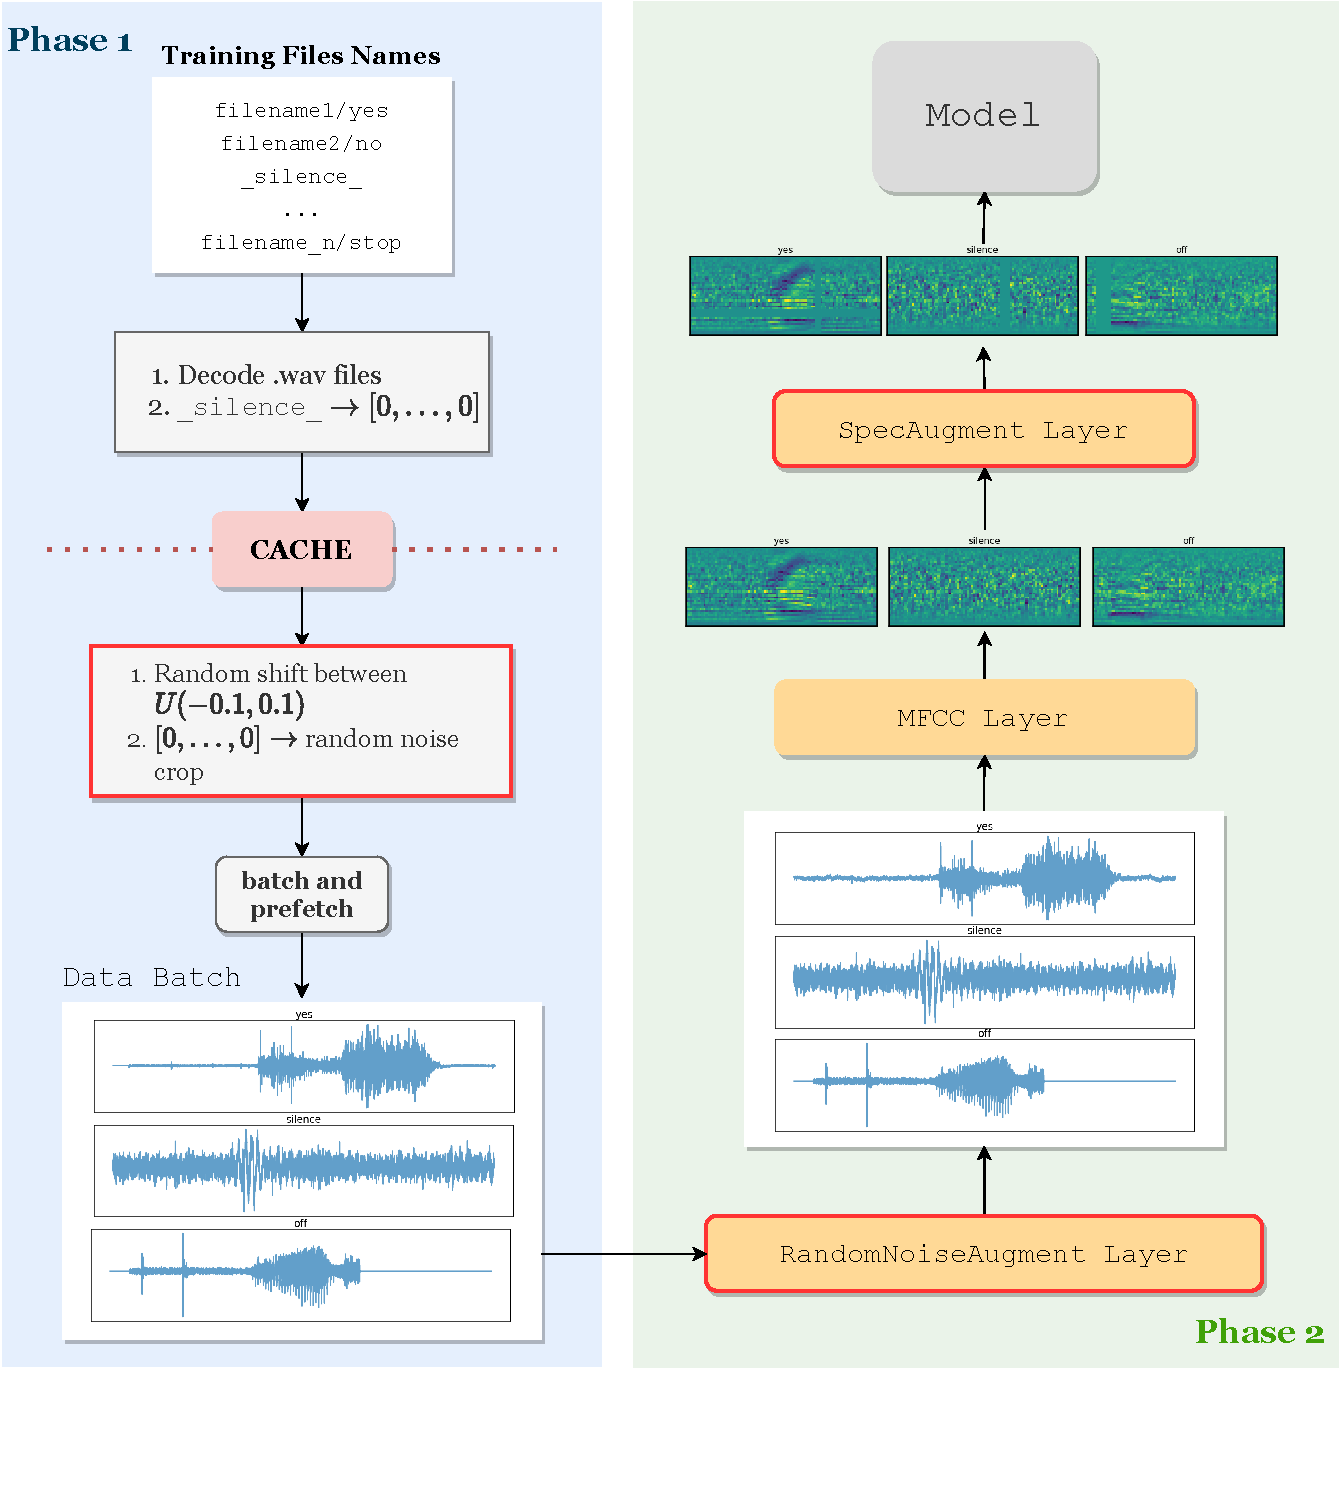
\includegraphics[width=0.99\linewidth]{imgs/input_pipeline_v3.pdf}
	%TODO: image is still wip
	\caption{Detailed description of the input pipeline for the training data. In the cache block, the data that was produced until that moment is saved to file. Each step which is performed before the caching operation happens only one time, during the first iteration of the dataset; on all the successive iterations, the data is read from the cached file. Boxes with the red outline denote data augmentation steps}
	\label{fig:inputpipeline}
\end{figure}





\subsection{Learning Framework}
\label{sec:learning_framework}

We now describe each proposed architecture, mainly using summary tables. Note that each RNN layer is bidirectional, and each CNN layer uses batch normalization before passing through the activation function. Also, the first layers of each model are the preprocessing layers discussed in the previous section; here we don't report them as they are not part of the real model architecture. In the tables we report with $m$ the number of output classes, which differ depending on the type of task. Finally, we denote with \say{Attention} the attention layer used by Att-RNN, while with \say{QAttention} we mean the attention layer introduced for SQAtt-RNN.

\subsubsection{\textbf{SimpleAtt}}
We propose this model as a baseline light weight model to see how its performances compare to more complex architectures. It's architecture is shown in Table \ref{tab:simpleatt_architecture}.

\begin{table}[h]
	\caption{Simple Attention RNN Architecture}
	\label{tab:simpleatt_architecture}
	\begin{tabular}{|c|c|c|c|c|c|c|}
		\hline
		layer type & $n$RNN & $n$MLP & $n$F & Fw & Fh & Act.    \\ \hline
		RNN (GRU)  & $64$   &      &    &    &    & tanh    \\ \hline
		Attention  &      &      &    &    &    &         \\ \hline
		Dense      &      & $128$  &    &    &    & ReLu    \\ \hline
		Dense      &      & $64$   &    &    &    & ReLu    \\ \hline
		Dense      &      & $m$  &    &    &    & Softmax \\ \hline
	\end{tabular}
\end{table}
\subsubsection{\textbf{Att-RNN}}
The baseline model, from \cite{attention2018andreade}. Architecture is shown in Table \ref{tab:attrnn_architecture}.

\begin{table}[h]
	\caption{Att-RNN Architecture}
	\label{tab:attrnn_architecture}
	\begin{tabular}{|c|c|c|c|c|c|c|}
	\hline
	layer type & $n$RNN & $n$MLP & $n$F & Fw & Fh & Act.    \\ \hline
	Conv       &      &      & $10$ & $5$  & $1$  & ReLu    \\ \hline
	Conv       &      &      & $1$  & $5$  & $1$  & ReLu    \\ \hline
	RNN (LSTM) & $128$  &      &    &    &    & tanh    \\ \hline
	RNN(LSTM)  & $128$  &      &    &    &    & tanh    \\ \hline
	Attention  &      &      &    &    &    &         \\ \hline
	Dense      &      & $64$   &    &    &    & ReLu    \\ \hline
	Dense      &      & $m$  &    &    &    & Softmax \\ \hline
\end{tabular}
\end{table}

\subsubsection{\textbf{SQAtt-RNN}}
Simple variation of Att-RNN, where the attention layer is modified in order return a new sequence. The idea is that the new returned sequence will constitute a richer representation of the input sequence. Architecture is shown in Table \ref{tab:sqattrnn_architecture}.

\begin{table}[h]
		\caption{SQAtt-RNN Architecture}
	\label{tab:sqattrnn_architecture}
	\begin{tabular}{|c|c|c|c|c|c|c|}
		\hline
		layer type & nRNN & nMLP & nF & Fw & Fh & Act.    \\ \hline
		Conv       &      &      & 10 & 5  & 1  & ReLu    \\ \hline
		Conv       &      &      & 1  & 5  & 1  & ReLu    \\ \hline
		RNN (GRU)  & 128  &      &    &    &    & tanh    \\ \hline
		RNN (GRU)  & 128  &      &    &    &    & tanh    \\ \hline
		QAttention &      &      &    &    &    &         \\ \hline
		RNN (GRU)  & 64   &      &    &    &    & tanh    \\ \hline
		Dense      &      & 64   &    &    &    & ReLu    \\ \hline
		Dense      &      & $m$  &    &    &    & Softmax \\ \hline
	\end{tabular}
\end{table}


Each model was trained for 30 epochs, using early stopping and reduce lr on plateau %TODO: spiegare bene

%Here you finally describe the learning strategy / algorithm that you conceived and used to solve the problem at stake. A good diagram to exemplify how learning is carried out is often very useful. In this section, you should describe the learning model, its parameters, any optimization over a given parameter set, etc. You can organize this section into \mbox{sub-sections}. You are free to choose the most appropriate structure.
%
%\begin{remark}
%Note that the diagram that you put here differs from that of Section~\ref{sec:processing_architecture} as here you show the details of how your learning framework, or the core of it, is built. In Section~\ref{sec:processing_architecture} you instead provide a high-level description of the involved processing blocks, i.e., you describe the {\it processing flow} and the rationale behind it.
%\end{remark}
%
%
%
